\documentclass[]{article}
\usepackage{lmodern}
\usepackage{amssymb,amsmath}
\usepackage{ifxetex,ifluatex}
\usepackage{bm}
\usepackage{soul}
\usepackage[color=yellow]{todonotes}
\usepackage{fixltx2e} % provides \textsubscript
\ifnum 0\ifxetex 1\fi\ifluatex 1\fi=0 % if pdftex
  \usepackage[T1]{fontenc}
  \usepackage[utf8]{inputenc}
  \usepackage{eurosym}
\else % if luatex or xelatex
  \ifxetex
    \usepackage{mathspec}
  \else
    \usepackage{fontspec}
  \fi
  \defaultfontfeatures{Ligatures=TeX,Scale=MatchLowercase}
  \newcommand{\euro}{€}
\fi
% use upquote if available, for straight quotes in verbatim environments
\IfFileExists{upquote.sty}{\usepackage{upquote}}{}
% use microtype if available
\IfFileExists{microtype.sty}{%
\usepackage{microtype}
\UseMicrotypeSet[protrusion]{basicmath} % disable protrusion for tt fonts
}{}
\usepackage[margin=1in]{geometry}
\usepackage{hyperref}
\hypersetup{unicode=true,
            pdftitle={1 Introduction to time series analysis},
            pdfauthor={Edward Ionides},
            pdfborder={0 0 0},
            breaklinks=true}
\urlstyle{same}  % don't use monospace font for urls
\usepackage{color}
\usepackage{fancyvrb}
\newcommand{\VerbBar}{|}
\newcommand{\VERB}{\Verb[commandchars=\\\{\}]}
\DefineVerbatimEnvironment{Highlighting}{Verbatim}{commandchars=\\\{\}}
% Add ',fontsize=\small' for more characters per line
\usepackage{framed}
\definecolor{shadecolor}{RGB}{248,248,248}
\newenvironment{Shaded}{\begin{snugshade}}{\end{snugshade}}
\newcommand{\KeywordTok}[1]{\textcolor[rgb]{0.13,0.29,0.53}{\textbf{#1}}}
\newcommand{\DataTypeTok}[1]{\textcolor[rgb]{0.13,0.29,0.53}{#1}}
\newcommand{\DecValTok}[1]{\textcolor[rgb]{0.00,0.00,0.81}{#1}}
\newcommand{\BaseNTok}[1]{\textcolor[rgb]{0.00,0.00,0.81}{#1}}
\newcommand{\FloatTok}[1]{\textcolor[rgb]{0.00,0.00,0.81}{#1}}
\newcommand{\ConstantTok}[1]{\textcolor[rgb]{0.00,0.00,0.00}{#1}}
\newcommand{\CharTok}[1]{\textcolor[rgb]{0.31,0.60,0.02}{#1}}
\newcommand{\SpecialCharTok}[1]{\textcolor[rgb]{0.00,0.00,0.00}{#1}}
\newcommand{\StringTok}[1]{\textcolor[rgb]{0.31,0.60,0.02}{#1}}
\newcommand{\VerbatimStringTok}[1]{\textcolor[rgb]{0.31,0.60,0.02}{#1}}
\newcommand{\SpecialStringTok}[1]{\textcolor[rgb]{0.31,0.60,0.02}{#1}}
\newcommand{\ImportTok}[1]{#1}
\newcommand{\CommentTok}[1]{\textcolor[rgb]{0.56,0.35,0.01}{\textit{#1}}}
\newcommand{\DocumentationTok}[1]{\textcolor[rgb]{0.56,0.35,0.01}{\textbf{\textit{#1}}}}
\newcommand{\AnnotationTok}[1]{\textcolor[rgb]{0.56,0.35,0.01}{\textbf{\textit{#1}}}}
\newcommand{\CommentVarTok}[1]{\textcolor[rgb]{0.56,0.35,0.01}{\textbf{\textit{#1}}}}
\newcommand{\OtherTok}[1]{\textcolor[rgb]{0.56,0.35,0.01}{#1}}
\newcommand{\FunctionTok}[1]{\textcolor[rgb]{0.00,0.00,0.00}{#1}}
\newcommand{\VariableTok}[1]{\textcolor[rgb]{0.00,0.00,0.00}{#1}}
\newcommand{\ControlFlowTok}[1]{\textcolor[rgb]{0.13,0.29,0.53}{\textbf{#1}}}
\newcommand{\OperatorTok}[1]{\textcolor[rgb]{0.81,0.36,0.00}{\textbf{#1}}}
\newcommand{\BuiltInTok}[1]{#1}
\newcommand{\ExtensionTok}[1]{#1}
\newcommand{\PreprocessorTok}[1]{\textcolor[rgb]{0.56,0.35,0.01}{\textit{#1}}}
\newcommand{\AttributeTok}[1]{\textcolor[rgb]{0.77,0.63,0.00}{#1}}
\newcommand{\RegionMarkerTok}[1]{#1}
\newcommand{\InformationTok}[1]{\textcolor[rgb]{0.56,0.35,0.01}{\textbf{\textit{#1}}}}
\newcommand{\WarningTok}[1]{\textcolor[rgb]{0.56,0.35,0.01}{\textbf{\textit{#1}}}}
\newcommand{\AlertTok}[1]{\textcolor[rgb]{0.94,0.16,0.16}{#1}}
\newcommand{\ErrorTok}[1]{\textcolor[rgb]{0.64,0.00,0.00}{\textbf{#1}}}
\newcommand{\NormalTok}[1]{#1}
\usepackage{graphicx,grffile}
\makeatletter
\def\maxwidth{\ifdim\Gin@nat@width>\linewidth\linewidth\else\Gin@nat@width\fi}
\def\maxheight{\ifdim\Gin@nat@height>\textheight\textheight\else\Gin@nat@height\fi}
\makeatother
% Scale images if necessary, so that they will not overflow the page
% margins by default, and it is still possible to overwrite the defaults
% using explicit options in \includegraphics[width, height, ...]{}
\setkeys{Gin}{width=\maxwidth,height=\maxheight,keepaspectratio}
\IfFileExists{parskip.sty}{%
\usepackage{parskip}
}{% else
\setlength{\parindent}{0pt}
\setlength{\parskip}{6pt plus 2pt minus 1pt}
}
\setlength{\emergencystretch}{3em}  % prevent overfull lines
\providecommand{\tightlist}{%
  \setlength{\itemsep}{0pt}\setlength{\parskip}{0pt}}
%\setcounter{secnumdepth}{0}
\setcounter{section}{1}
% Redefines (sub)paragraphs to behave more like sections
\ifx\paragraph\undefined\else
\let\oldparagraph\paragraph
\renewcommand{\paragraph}[1]{\oldparagraph{#1}\mbox{}}
\fi
\ifx\subparagraph\undefined\else
\let\oldsubparagraph\subparagraph
\renewcommand{\subparagraph}[1]{\oldsubparagraph{#1}\mbox{}}
\fi

%%% Use protect on footnotes to avoid problems with footnotes in titles
\let\rmarkdownfootnote\footnote%
\def\footnote{\protect\rmarkdownfootnote}

%%% Change title format to be more compact
\usepackage{titling}

% Create subtitle command for use in maketitle
\newcommand{\subtitle}[1]{
  \posttitle{
    \begin{center}\large#1\end{center}
    }
}

\setlength{\droptitle}{-2em}
  \title{1. Introduction to time series analysis}
  \pretitle{\vspace{\droptitle}\centering\huge}
  \posttitle{\par}
  \author{Edward Ionides}
  \preauthor{\centering\large\emph}
  \postauthor{\par}
  \predate{\centering\large\emph}
  \postdate{\par}
  \date{1/03/2018}


\begin{document}
\maketitle

{
\setcounter{tocdepth}{2}
\tableofcontents
}
\newcommand\prob{\mathbb{P}}
\newcommand\E{\mathbb{E}}
\newcommand\SE{\mathrm{SE}}
\newcommand\var{\mathrm{Var}}
\newcommand\cov{\mathrm{Cov}}
\newcommand\loglik{\ell}
\newcommand\R{\mathbb{R}}
\newcommand\data[1]{#1^*}
\newcommand\estimate[1]{\data{#1}}
\newcommand\predict[1]{#1^{P*}}
\newcommand\given{\, ; \,}
\newcommand\transpose{\scriptsize{T}}





\begin{center}\rule{0.5\linewidth}{\linethickness}\end{center}

\begin{center}\rule{0.5\linewidth}{\linethickness}\end{center}

Objectives for this chapter

\begin{enumerate}
\def\labelenumi{\arabic{enumi}.}
\item
  Discuss some basic motivations for the topic of time series analysis.
\item
  Introduce some fundamental concepts for time series analysis:
  stationarity, autocorrelation, autoregressive models, moving average
  models, autoregressive-moving average (ARMA) models, state-space
  models. These will be covered in more detail later.
\item
  Develop the computational framework for this course:

  \begin{itemize}
  \tightlist
  \item
    R and Rmarkdown for data analysis and reproducible documents
  \item
    Source code sharing using git.
  \end{itemize}
\end{enumerate}

\begin{center}\rule{0.5\linewidth}{\linethickness}\end{center}

\begin{center}\rule{0.5\linewidth}{\linethickness}\end{center}

\subsection{Overview}\label{overview}

\begin{itemize}
\item
  Time series data are, simply, data collected at many different times.
\item
  This is a common type of data! Observations at similar time points are
  often more similar than more distant observations.
\item
  This immediately forces us to think beyond the independent,
  identically distributed assumptions fundamental to much basic
  statistical theory and practice.
\item
  Time series dependence is an introduction to more complicated
  dependence structures: space, space/time, networks
  (social/economic/communication), \ldots{}
\end{itemize}

\begin{center}\rule{0.5\linewidth}{\linethickness}\end{center}

\begin{center}\rule{0.5\linewidth}{\linethickness}\end{center}

\subsubsection{Looking for trends and relationships in dependent
data}\label{looking-for-trends-and-relationships-in-dependent-data}

\begin{itemize}
\item
  The first half of this course focuses on:

  \begin{enumerate}
  \def\labelenumi{\arabic{enumi}.}
  \item
    Quantifying dependence in time series data.
  \item
    Finding statistical arguments for the presence or absence of
    associations that are valid in situations with dependence.
  \end{enumerate}
\item
  Example questions: Does Michigan show evidence for global warming?
  Does Michigan follow global trends, or is there evidence for regional
  variation? What is a good prediction interval for weather in the next
  year or two?
\end{itemize}

\begin{center}\rule{0.5\linewidth}{\linethickness}\end{center}

\begin{center}\rule{0.5\linewidth}{\linethickness}\end{center}

\subsubsection{Modeling and statistical inference for dynamic
systems}\label{modeling-and-statistical-inference-for-dynamic-systems}

\begin{itemize}
\item
  The second half of this course focuses on:

  \begin{enumerate}
  \def\labelenumi{\arabic{enumi}.}
  \item
    Building models for dynamic systems, which may or may not be linear
    and Gaussian.
  \item
    Using time series data to carry out statistical inference on these
    models.
  \end{enumerate}
\item
  Example questions: Can we develop a better model for understanding
  variability of financial markets (known in finance as volatility)? How
  do we assess our model and decide whether it is indeed an improvement?
\end{itemize}

\begin{center}\rule{0.5\linewidth}{\linethickness}\end{center}

\begin{center}\rule{0.5\linewidth}{\linethickness}\end{center}

\subsection{A simple example: Winter in
Michigan}\label{a-simple-example-winter-in-michigan}

The previous winter was mild by Michigan standards. What should we
expect this year? Is there a noticeable trend? Let's look at some data.

I downloaded from
\href{https://www.usclimatedata.com/climate/ann-arbor/michigan/united-states/usmi0028}{www.usclimatedata.com}
and put in \url{ann_arbor_weather.csv}.

\begin{itemize}
\item
  You can get this file from the course website
  (\url{http://ionides.github.io/531w18}).
\item
  Better, you can set up a local git repository that will give you an
  up-to-date copy of all the data, notes, code, homeworks and solutions
  for this course. More on this later.
\end{itemize}

\begin{Shaded}
\begin{Highlighting}[]
\NormalTok{y <-}\StringTok{ }\KeywordTok{read.table}\NormalTok{(}\DataTypeTok{file=}\StringTok{"ann_arbor_weather.csv"}\NormalTok{,}\DataTypeTok{header=}\DecValTok{1}\NormalTok{)}
\end{Highlighting}
\end{Shaded}

Here, I'm using R Markdown to combine source code with text. This gives
a nice way to generate statistical analysis that is

\begin{enumerate}
\def\labelenumi{\arabic{enumi}.}
\item
  Reproducible,
\item
  Easily modified or extended.
\end{enumerate}

These two properties are useful for developing your own statistical
research projects. Also, they are useful for teaching and learning
statistical methodology, since they make it easy for you to replicate
and adapt analysis presented in class.

\begin{center}\rule{0.5\linewidth}{\linethickness}\end{center}

\begin{center}\rule{0.5\linewidth}{\linethickness}\end{center}

\subsubsection{Question: How many of you already know R
Markdown?}\label{question-how-many-of-you-already-know-r-markdown}

\begin{center}\rule{0.5\linewidth}{\linethickness}\end{center}

\begin{center}\rule{0.5\linewidth}{\linethickness}\end{center}

First, let's get some basic idea what's in our dataset. \texttt{str}
summarizes the structure of the data:

\begin{Shaded}
\begin{Highlighting}[]
\KeywordTok{str}\NormalTok{(y)}
\end{Highlighting}
\end{Shaded}

\begin{verbatim}
## 'data.frame':    118 obs. of  12 variables:
##  $ Year     : int  1900 1901 1902 1903 1904 1905 1906 1907 1908 1909 ...
##  $ Low      : num  -7 -7 -4 -7 -11 -3 11 -8 -8 -1 ...
##  $ High     : num  50 48 41 50 38 47 62 61 42 61 ...
##  $ Hi_min   : num  36 37 27 36 31 32 53 38 32 50 ...
##  $ Lo_max   : num  12 20 11 12 6 14 20 11 15 13 ...
##  $ Avg_min  : num  18 17 15 15.1 8.2 10.9 25.8 17.2 17.6 20 ...
##  $ Avg_max  : num  34.7 31.8 30.4 29.6 22.9 25.9 38.8 31.8 28.9 34.7 ...
##  $ Mean     : num  26.3 24.4 22.7 22.4 15.3 18.4 32.3 24.5 23.2 27.4 ...
##  $ Precip   : num  1.06 1.45 0.6 1.27 2.51 1.64 1.91 4.68 1.06 2.5 ...
##  $ Snow     : num  4 10.1 6 7.3 11 7.9 3.6 16.1 4.3 8.7 ...
##  $ Hi_Pricip: num  0.28 0.4 0.25 0.4 0.67 0.84 0.43 1.27 0.63 1.27 ...
##  $ Hi_Snow  : num  1.1 3.2 2.5 3.2 2.1 2.5 2 5 1.3 7 ...
\end{verbatim}

Let's focus on \texttt{Low}, which is the lowest temperature, in
Fahrenheit, for January of each year.

\begin{itemize}
\item
  There are practical reasons to understand the expected (i.e., mean)
  low temperature and the annual variation around this. Reasons to do
  this could be

  \begin{itemize}
  \item
    Agriculture: can I grow ginseng in Ann Arbor?
  \item
    Energy: assess the cost-effectiveness of installing extra home
    insulation.
  \item
    Lifestyle: Should I move to Minneapolis, or Berlin, or Beijing?
  \end{itemize}
\item
  Also, we could develop our analysis to look for evidence of climate
  change.
\item
  As statisticians, we want an uncertainty estimate. We want to know how
  reliable our estimate is, since it is based on only a limited amount
  of data.
\item
  The data are \(y^*_1,\dots,y^*_N\), which we also write as
  \(\data{y_{1:N}}\).
\item
  Basic estimates of the mean and standard deviation are
  \[\estimate{\hat\mu_1}= \frac{1}{N}\sum_{n=1}^Ny^*_n, \hspace{2cm}
  \estimate{\hat\sigma_1}= \sqrt{\frac{1}{N-1}\sum_{n=1}^N(y^*_n-\hat{\mu_1})^2}.\]
\item
  We are being pedantic about adding the asterisks to denote that
  \(\estimate{\hat\mu_1}\) is the \textbf{estimate} derived from
  evaluating the \textbf{estimator} \(\hat\mu_1\) using the data
  \(\data{y_{1:N}}\).
\item
  This suggests an approximate confidence interval for \(\mu\) of
  \(\estimate{\hat\mu_1} \pm 1.96\, \estimate{\hat\sigma_1}/\sqrt{N}\),
\item
  1955 has missing data, coded as \texttt{NA}, requiring a minor
  modification. So, we compute \(\estimate{\hat\mu_1}\) and
  \(\SE_1=\estimate{\hat\sigma_1}/\sqrt{N}\) as
\end{itemize}

\begin{Shaded}
\begin{Highlighting}[]
\NormalTok{mu1 <-}\StringTok{ }\KeywordTok{mean}\NormalTok{(y}\OperatorTok{\$}\NormalTok{Low,}\DataTypeTok{na.rm=}\OtherTok{TRUE}\NormalTok{)}
\NormalTok{se1 <-}\StringTok{ }\KeywordTok{sd}\NormalTok{(y}\OperatorTok{\$}\NormalTok{Low,}\DataTypeTok{na.rm=}\OtherTok{TRUE}\NormalTok{)}\OperatorTok{/}\KeywordTok{sqrt}\NormalTok{(}\KeywordTok{sum}\NormalTok{(}\OperatorTok{!}\KeywordTok{is.na}\NormalTok{(y}\OperatorTok{\$}\NormalTok{Low)))}
\KeywordTok{cat}\NormalTok{(}\StringTok{"mu1 ="}\NormalTok{, mu1, }\StringTok{",  se1 ="}\NormalTok{, se1, }\StringTok{"}\CharTok{\textbackslash{}n}\StringTok{"}\NormalTok{)}
\end{Highlighting}
\end{Shaded}

\begin{verbatim}
## mu1 = -2.717949 ,  se1 = 0.675042
\end{verbatim}

\begin{itemize}
\tightlist
\item
  Note that \(\SE_1\) is also an estimate. We could therefore write
  \(\estimate{\SE_1}\), but here there is less room for
  misinterpretation.
\end{itemize}

\begin{center}\rule{0.5\linewidth}{\linethickness}\end{center}

\begin{center}\rule{0.5\linewidth}{\linethickness}\end{center}

\subsubsection{\texorpdfstring{Question: What are the assumptions behind
the resulting confidence interval,
\(-2.72 \pm 1.32\).}{Question: What are the assumptions behind the resulting confidence interval, -2.72 \textbackslash{}pm 1.32.}}\label{question-what-are-the-assumptions-behind-the-resulting-confidence-interval--2.72-pm-1.32.}

\subsubsection{Question: When, in practice, is it reasonable to present
this confidence interval? Is it reasonable
here?}\label{question-when-in-practice-is-it-reasonable-to-present-this-confidence-interval-is-it-reasonable-here}

\subsubsection{Question: How would you
proceed?}\label{question-how-would-you-proceed}

\begin{center}\rule{0.5\linewidth}{\linethickness}\end{center}

\begin{center}\rule{0.5\linewidth}{\linethickness}\end{center}

\subsubsection{Some data analysis}\label{some-data-analysis}

\begin{itemize}
\tightlist
\item
  The first rule of data analysis is to plot the data in as many ways as
  you can think of! For time series, we usually start with a time plot
\end{itemize}

\begin{Shaded}
\begin{Highlighting}[]
\KeywordTok{plot}\NormalTok{(Low}\OperatorTok{~}\NormalTok{Year,}\DataTypeTok{data=}\NormalTok{y,}\DataTypeTok{ty=}\StringTok{"l"}\NormalTok{)}
\end{Highlighting}
\end{Shaded}

\begin{center}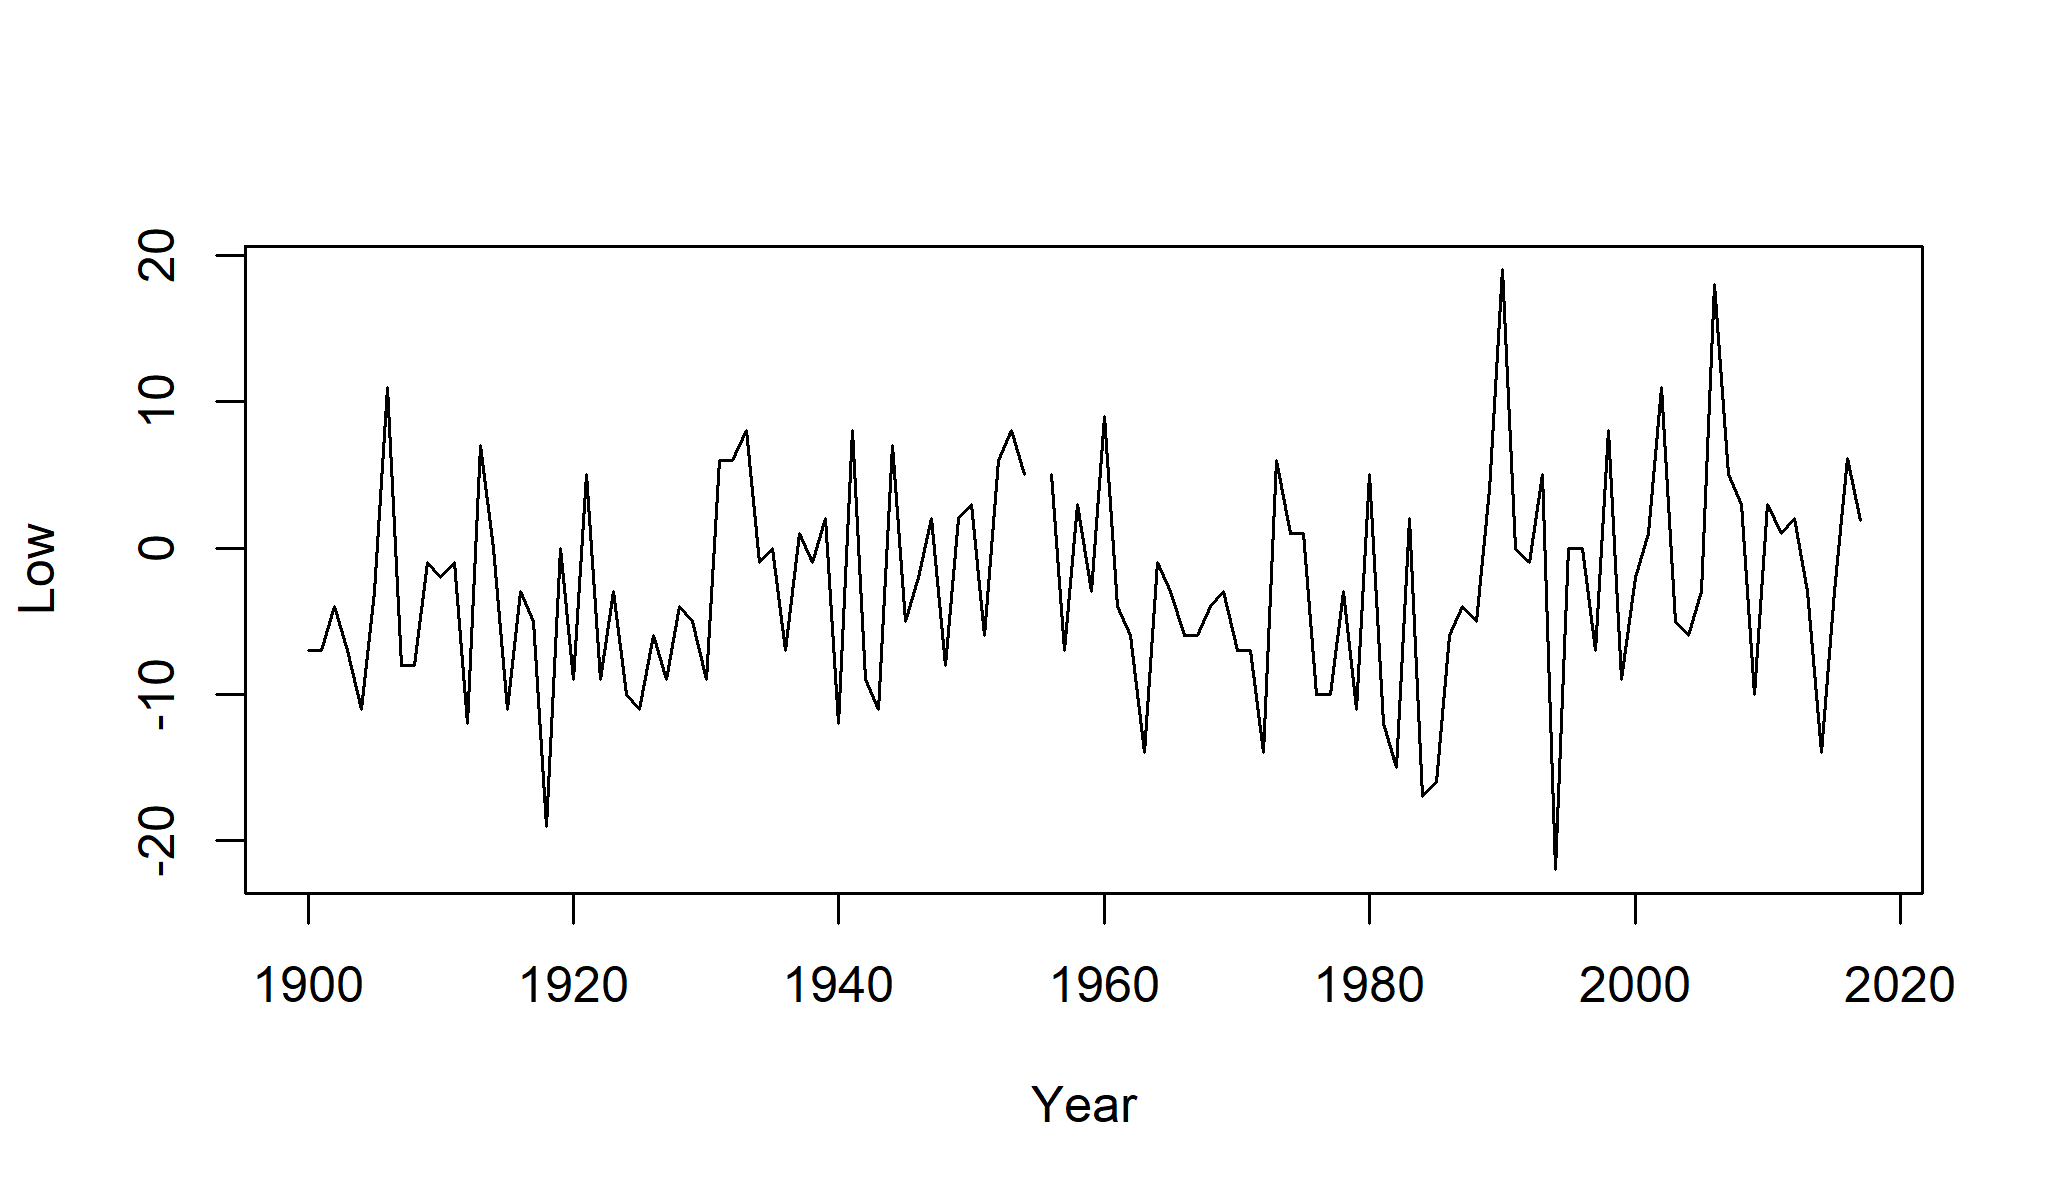
\includegraphics{figure/intro-weather_plot-1} \end{center}

\begin{itemize}
\item
  Another simple thing to do is to fit an \textbf{autoregressive-moving
  average} (ARMA) model. We'll look at ARMA models in much more detail
  later in the course.
\item
  Let's fit an ARMA model given by
  \[ Y_n = \mu + \alpha(Y_{n-1}-\mu) + \epsilon_n + \beta \epsilon_{n-1}.\]
  This has a one-lag autoregressive term, \(\alpha(Y_{n-1}-\mu)\), and a
  one-lag moving average term, \(\beta \epsilon_{n-1}\). It is therefore
  called an ARMA(1,1) model. These lags give the model some time
  dependence.

  \begin{itemize}
  \item
    If \(\alpha=\beta=0\), we get back to the basic independent model,
    \(Y_n = \mu + \epsilon_n\).
  \item
    If \(\alpha=0\) we have a moving average model with one lag, MA(1).
  \item
    If \(\beta=0\), we have an autoregressive model with one lag, AR(1).
  \end{itemize}
\item
  We model \(\epsilon_1\dots,\epsilon_N\) to be an independent,
  identically distributed sequence. To be concrete, let's specify a
  model where they are normally distributed with mean zero and variance
  \(\sigma^2\).
\item
  A note on notation:

  \begin{itemize}
  \item
    In this course, capital Roman letters, e.g., \(X\), \(Y\), \(Z\),
    denote random variables. We may also use \(\epsilon\), \(\eta\),
    \(\xi\), \(\zeta\) for random noise processes. Thus, these symbols
    are used to build models.
  \item
    We use lower case Roman letters (\(x\), \(y\), \(z\), \(\dots\)) to
    denote fixed numbers.
  \item
    When fixed numbers are data, or are derived from data, we will often
    add an asterisk (\(x^*\), \(y^*\), \(\dots\)). A quantity derived
    from data is called a \textbf{statistic}.
  \item
    ``We must be careful not to confuse data with the abstractions we
    use to analyze them.'' (William James, 1842-1910).
  \item
    Other Greek letters will usually be parameters, i.e., real numbers
    that form part of the model.
  \end{itemize}
\item
  We can readily fit the ARMA(1,1) model by maximum likelihood,
\end{itemize}

\begin{Shaded}
\begin{Highlighting}[]
\NormalTok{arma11 <-}\StringTok{ }\KeywordTok{arima}\NormalTok{(y}\OperatorTok{\$}\NormalTok{Low, }\DataTypeTok{order=}\KeywordTok{c}\NormalTok{(}\DecValTok{1}\NormalTok{,}\DecValTok{0}\NormalTok{,}\DecValTok{1}\NormalTok{))}
\end{Highlighting}
\end{Shaded}

We can see a summary of the fitted model, where \(\alpha\) is called
\texttt{ar1}, \(\beta\) is called \texttt{ma1}, and \(\mu\) is called
\texttt{intercept}.

\begin{Shaded}
\begin{Highlighting}[]
\NormalTok{arma11}
\end{Highlighting}
\end{Shaded}

\begin{verbatim}
## 
## Call:
## arima(x = y$Low, order = c(1, 0, 1))
## 
## Coefficients:
##          ar1      ma1  intercept
##       0.8400  -0.7972    -2.7103
## s.e.  0.2424   0.2661     0.8387
## 
## sigma^2 estimated as 52.53:  log likelihood = -397.77,  aic = 803.55
\end{verbatim}

\todo[inline]{SE's created by taking fisher information matrix at MLE}

We will write the ARMA(1,1) estimate of \(\mu\) as
\(\estimate{\hat\mu_2}\), and its standard error as \(\SE_2\). Some
poking around is required to extract the quantities of primary interest
from the fitted ARMA model in R.

\begin{Shaded}
\begin{Highlighting}[]
\KeywordTok{names}\NormalTok{(arma11)}
\end{Highlighting}
\end{Shaded}

\begin{verbatim}
##  [1] "coef"      "sigma2"    "var.coef"  "mask"      "loglik"   
##  [6] "aic"       "arma"      "residuals" "call"      "series"   
## [11] "code"      "n.cond"    "nobs"      "model"
\end{verbatim}

\begin{Shaded}
\begin{Highlighting}[]
\NormalTok{mu2 <-}\StringTok{ }\NormalTok{arma11}\OperatorTok{\$}\NormalTok{coef[}\StringTok{"intercept"}\NormalTok{]}
\NormalTok{se2 <-}\StringTok{ }\KeywordTok{sqrt}\NormalTok{(arma11}\OperatorTok{\$}\NormalTok{var.coef[}\StringTok{"intercept"}\NormalTok{,}\StringTok{"intercept"}\NormalTok{])}
\KeywordTok{cat}\NormalTok{(}\StringTok{"mu2 ="}\NormalTok{, mu2, }\StringTok{",  se2 ="}\NormalTok{, se2, }\StringTok{"}\CharTok{\textbackslash{}n}\StringTok{"}\NormalTok{)}
\end{Highlighting}
\end{Shaded}

\begin{verbatim}
## mu2 = -2.710296 ,  se2 = 0.8386897
\end{verbatim}

\begin{itemize}
\item
  We see that the two estimates, \(\estimate{\hat\mu_1}=-2.72\) and
  \(\estimate{\hat\mu_2}=-2.71\), are close. However, \(\SE_1=0.68\) is
  an underestimate of error, compared to the better estimate
  \(\SE_2=0.84\). The naive standard error needs to be inflated by
  \(100(\SE_2/\SE_1-1)=\) 24.2 percent.
\item
  Exactly how the ARMA(1,1) model is fitted and the standard errors
  computed will be covered later.
\item
  We should do \textbf{diagnostic analysis}. The first thing to do is to
  look at the residuals. For an ARMA model, the residual \(\data{r_n}\)
  at time \(t_n\) is defined to be the difference between the data,
  \(\data{y_n}\), and a one-step ahead prediction of \(\data{y_n}\)
  based on \(\data{y_{1:n-1}}\), written as \(\predict{y_n}\). From the
  ARMA(1,1) definition,
  \[ Y_n = \mu + \alpha(Y_{n-1}-\mu) + \epsilon_n + \beta \epsilon_{n-1},\]
  a basic one-step-ahead predicted value corresponding to parameter
  estimates \(\estimate{\hat\mu}\) and \(\estimate{\hat\alpha}\) could
  be
  \[\predict{y_n} = \estimate{\hat{\mu}} + \estimate{\hat{\alpha}}(\data{y_{n-1}}-\estimate{\hat{\mu}}).\]
  A so-called residual time series, \(\{\data{r_n}\}\), is then given by
  \[ \data{r_n} = \data{y_n} - \predict{y_n}.\] In fact, R does
  something slightly more sophisticated.
\end{itemize}

\begin{Shaded}
\begin{Highlighting}[]
\KeywordTok{plot}\NormalTok{(arma11}\OperatorTok{\$}\NormalTok{resid)}
\end{Highlighting}
\end{Shaded}

\begin{center}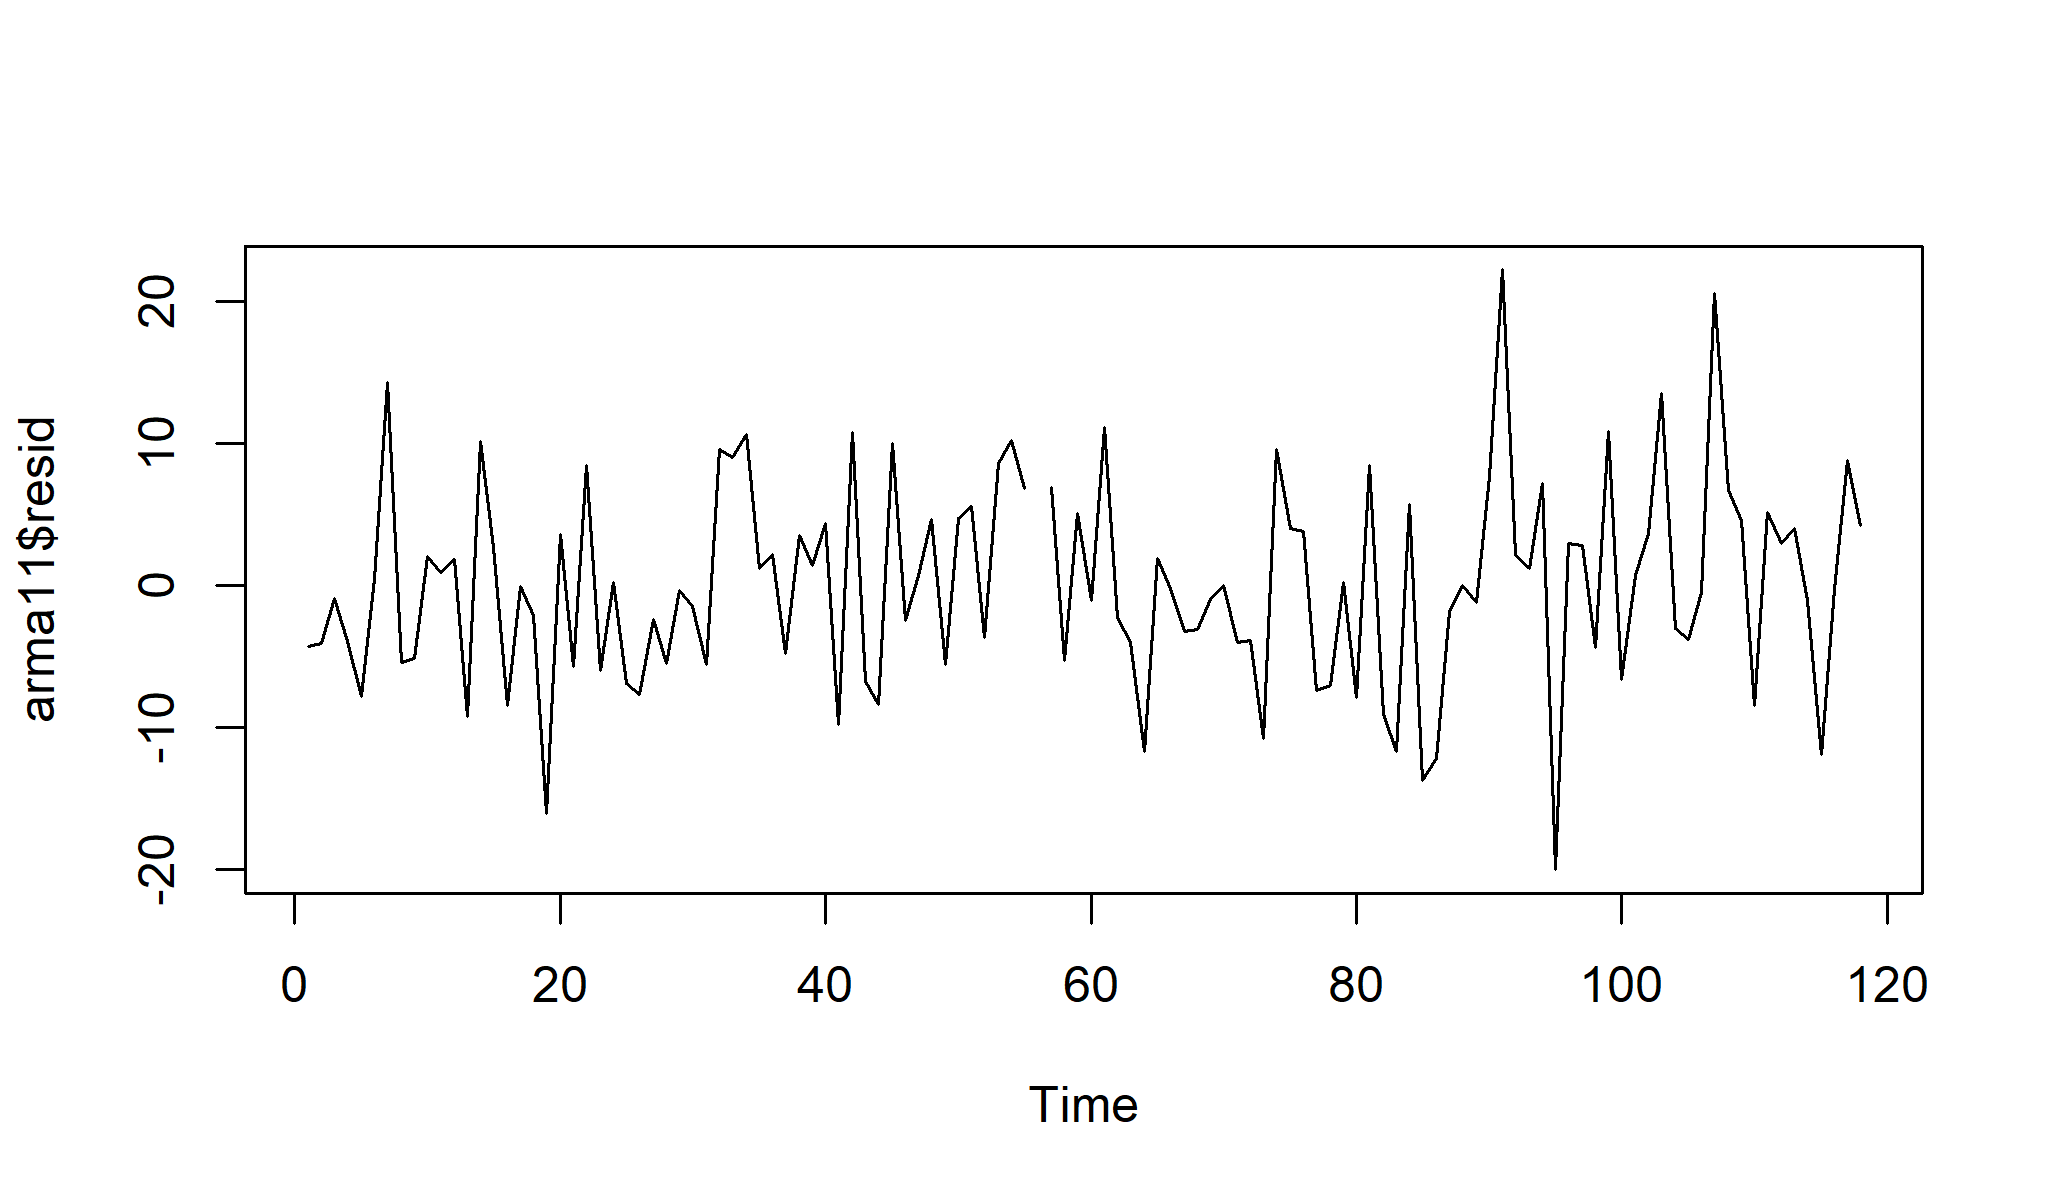
\includegraphics{figure/intro-arma_diag-1} \end{center}

\begin{itemize}
\tightlist
\item
  We see that there seems to be some slow variation in the residuals,
  over a decadal time scale. However, the residuals are close to
  uncorrelated, as we can check by plotting their pairwise sample
  correlations at a range of lags. This is called the \hl{sample
  autocorrelation function, or sample ACF}, which can be computed at each
  lag \(h\) for the residual time series \(\{\data{r_n}\}\) as
  \[ \estimate{\mathrm{ACF}}(h) = \frac{\frac{1}{N}\sum_{n=1}^{N-h} \data{r_n} \, \data{r_{n+h}}}
  {\frac{1}{N}\sum_{n=1}^{N} (\data{r_{n}})^2}.\] We will discuss the
  sample ACF at greater length later.
\end{itemize}

\begin{Shaded}
\begin{Highlighting}[]
\KeywordTok{acf}\NormalTok{(arma11}\OperatorTok{\$}\NormalTok{resid,}\DataTypeTok{na.action=}\NormalTok{na.pass)}
\end{Highlighting}
\end{Shaded}

\begin{center}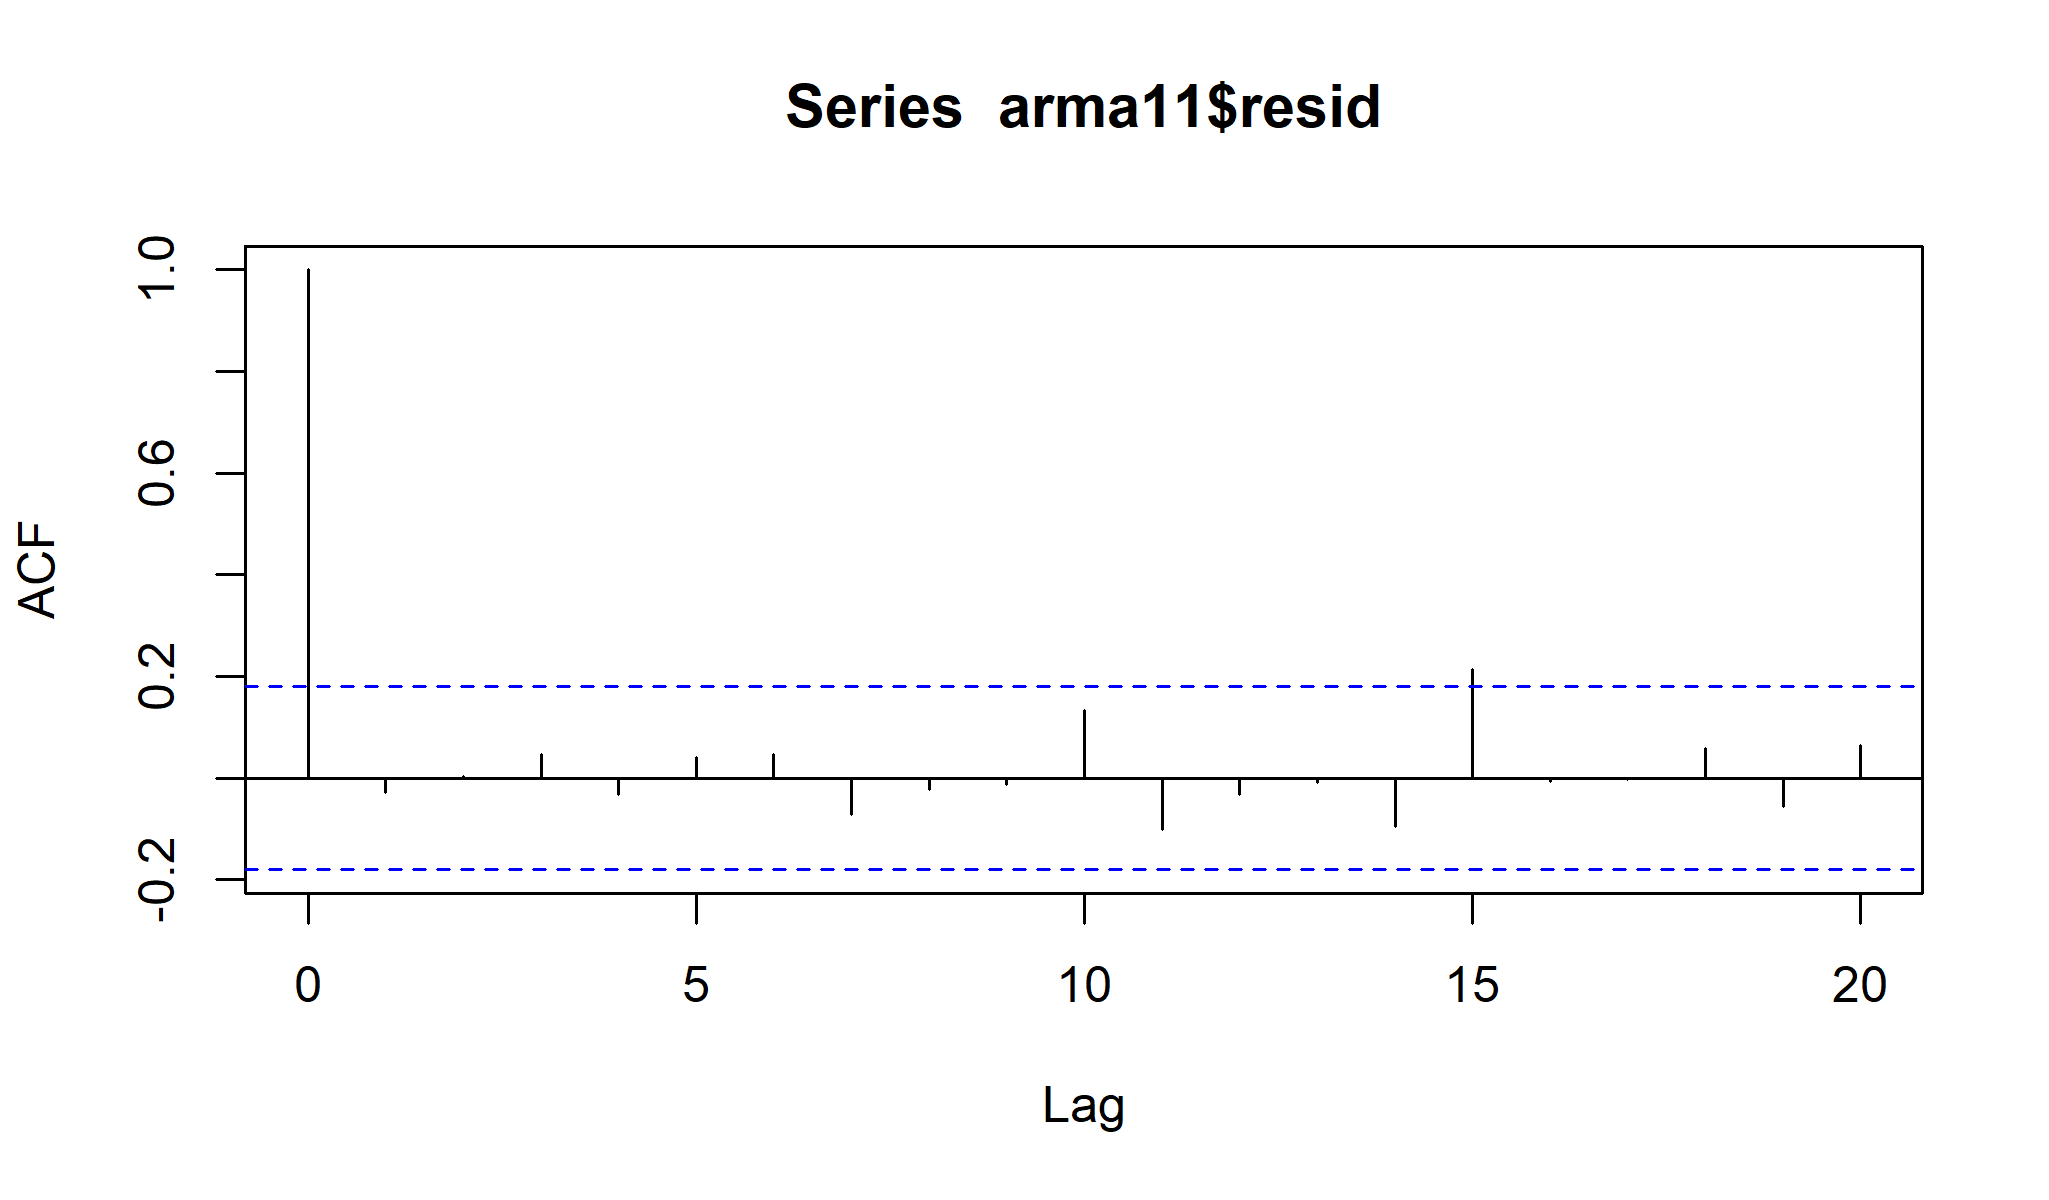
\includegraphics{figure/intro-acf-1} \end{center}

\begin{itemize}
\item
  This shows not much sign of autocorrelation. In other words, fitting
  \hl{ARMA models is unlikely to be a good way to describe the slow
  variation} present in the residuals of the ARMA(1,1) model.
\item
  There is probably some room for improvement over \(\SE_2\), which
  might lead to a somewhat larger standard error estimate.
\item
  Although this is just a toy example, the issue of inadequate models
  giving poor statistical uncertainty estimates is a major concern
  whenever working with time series data.
\item
  Usually, omitted dependency in the model will give overconfident (too
  small) standard errors.

  \begin{itemize}
  \item
    This leads to scientific reproducibility problems, where chance
    variation is too often assigned statistical significance.
  \item
    It can also lead to improper pricing of risk in financial markets, a
    factor in the US financial crisis of 2007-2008.
  \end{itemize}
\end{itemize}

\begin{center}\rule{0.5\linewidth}{\linethickness}\end{center}

\begin{center}\rule{0.5\linewidth}{\linethickness}\end{center}

\subsection{Models dynamic systems: State-space
models}\label{models-dynamic-systems-state-space-models}

\begin{itemize}
\item
  Scientists and engineers often have equations in mind to describe a
  system they're interested in.
\item
  Often, we have a model for how the state of a stochastic dynamic
  system evolves through time, and another model for how imperfect
  measurements on this system gives rise to a time series of
  observations.
\item
  This is called a \hl{\textbf{state-space model}}.
\item
  The \hl{\textbf{state} models the quantities that we think determine how
  the system changes with time}. However, these idealized state variables
  are not usually directly and perfectly measurable.
\item
  Statistical analysis of time series data on a system should be able to

  \begin{enumerate}
  \def\labelenumi{\arabic{enumi}.}
  \item
    Help scientists choose between rival hypotheses.
  \item
    Estimate unknown parameters in the model equations.
  \end{enumerate}
\item
  We will look at examples from a wide range of scientific applications.
  The dynamic model may be linear or nonlinear, Gaussian or
  non-Gaussian. Here is an example from finance.
\end{itemize}

\begin{center}\rule{0.5\linewidth}{\linethickness}\end{center}

\begin{center}\rule{0.5\linewidth}{\linethickness}\end{center}

\subsubsection{Fitting a model for volatility of a stock market
index}\label{fitting-a-model-for-volatility-of-a-stock-market-index}

\begin{itemize}
\item
  Let \(\{y^*_n,n=1,\dots,N\}\) be the daily returns on a stock market
  index, such as the S\&P 500.
\item
  Since the stock market is notoriously unpredictable, it is often
  unproductive to predict the mean of the returns and instead there is
  much emphasis on predicting the variability of the returns, known as
  the \textbf{volatility}.
\item
  Volatility is critical to assessing the risk of financial investments.
\item
  Financial mathematicians have postulated the following model. We will
  not work on understanding it right now. The relevant point here is
  that investigators often find it useful to write down models for how a
  dynamic system progresses through time, and this gives rise to the
  time series analysis goals of estimating unknown parameters and
  assessing how successfully the fitted model describes the data.
\end{itemize}

\[
\begin{aligned} Y_n &= \exp\left\{\frac{H_n}{2}\right\} \epsilon_n, \\
H_n &= \mu_h(1-\phi) + \phi H_{n-1} \\
&\quad\quad +  Y_{n-1}\sigma_\eta\sqrt{1-\phi^2}\tanh(G_{n-1}+\nu_n)\exp\left\{\frac{-H_{n-1}}{2}\right\} + \omega_n,\\
G_n &= G_{n-1}+\nu_n,
\end{aligned}
\]

\begin{itemize}
\item
  \(\{\epsilon_n\}\) is an iid \(N(0,1)\) sequence, \(\{\nu_n\}\) is an
  iid \(N(0,\sigma_{\nu}^2)\) sequence, and \(\{\omega_n\}\) is an iid
  \(N(0,\sigma_\omega^2)\) sequence.
\item
  \(H_n\) represents the volatility at time \(t_n\). Volatility is
  unobserved; we only get to observe the return, \(Y_n\).
\item
  \(G_n\) is a slowly-varying process that regulates \(H_n\).
\item
  \(H_n\) has auto-regressive behavior and dependence on the previous
  return, \(Y_{n-1}\), as well as being driven by \(G_n\).
\end{itemize}

This is an example of a \hl{mechanistic model, where scientific or
engineering considerations lead to a model of interest}. Now there is
data and a model of interest, it is time to recruit a statistician!
(Statisticians can have roles to play in data collection and model
development, as well.)

\begin{center}\rule{0.5\linewidth}{\linethickness}\end{center}

\begin{center}\rule{0.5\linewidth}{\linethickness}\end{center}

\subsubsection{Relevant questions to be addressed using methodology
covered later in the
course}\label{relevant-questions-to-be-addressed-using-methodology-covered-later-in-the-course}

\begin{enumerate}
\def\labelenumi{\arabic{enumi}.}
\item
  How can we get good estimates of the parameters, \(\mu_h\), \(\phi\),
  \(\sigma_\nu\), \(\sigma_\omega\), together with their uncertainties?
\item
  Does this model fit better than alternative models? So far as it does,
  what have we learned?
\end{enumerate}

\begin{center}\rule{0.5\linewidth}{\linethickness}\end{center}

\begin{center}\rule{0.5\linewidth}{\linethickness}\end{center}

\subsubsection{Outline of a solution}\label{outline-of-a-solution}

\begin{itemize}
\item
  Likelihood-based inference for this partially observed stochastic
  dynamic system is possible, and enables addressing these questions
  (Bretó 2014).
\item
  Carrying out such an analysis is facilitated by recent advances in
  algorithms (Ionides et al. 2015).
\item
  The R package system and R markdown make state-of-the-art statistical
  analysis reproducible and extendable by Masters level statisticians!
  For example, with a modest amount of effort, you could run the code
  given in the
  \href{http://dept.stat.lsa.umich.edu/~ionides/tutorials/sp500/sp500.html}{online
  tutorial} reproducing part of Bretó (2014). We will look more at these
  data and models later.
\end{itemize}

\begin{center}\rule{0.5\linewidth}{\linethickness}\end{center}

\begin{center}\rule{0.5\linewidth}{\linethickness}\end{center}

\subsection{Internet repositories for collaboration and open-source
research: git and
github}\label{internet-repositories-for-collaboration-and-open-source-research-git-and-github}

\begin{itemize}
\item
  Git is currently the dominant tool for managing, developing and
  sharing code within the computational sciences and industry. Github is
  the largest git-based internet repository, but others (such as
  bitbucket) also use git, and it can be useful to use git to build a
  local repository on your own computer.
\item
  This course will benefit directly from using git, since it provides a
  convenient way to manage the code, data, notes and other files
  involved in the course.
\item
  Also, you will be practicing a skill that will likely be useful for
  future work.
\item
  Our immediate goals are

  \begin{enumerate}
  \def\labelenumi{\roman{enumi}.}
  \item
    Learn some ways to think about what a git repository is and how it
    works.
  \item
    Go through the process of downloading a github repository, editing
    it, and uploading the changes.
  \end{enumerate}
\item
  This introduction uses material from Karl Broman's practical and
  minimal git/github tutorial
  (\href{http://kbroman.org/github_tutorial/}{kbroman.org/github\_tutorial}).
  A deeper, more technical tutorial is
  \href{https://www.atlassian.com/git/tutorials/}{www.atlassian.com/git/tutorials}.
\item
  This course will require only basic familiarity with git. Indeed, all
  the materials will be on the website so it is not essential that you
  use git at all. However, keeping a local copy of the course git
  project is a good way to maintain up-to-date copies of all the files.
  Also, you may find additional features of git to be useful, such as
  making pull requests with corrections or improvements to the notes!
\end{itemize}

\begin{center}\rule{0.5\linewidth}{\linethickness}\end{center}

\begin{center}\rule{0.5\linewidth}{\linethickness}\end{center}

\subsubsection{Getting started with git and
github}\label{getting-started-with-git-and-github}

\begin{enumerate}
\def\labelenumi{\arabic{enumi}.}
\item
  Get an account on \href{http://github.com}{github}.
\item
  If you are on a Mac or Linux machine, git will likely be installed
  already. Otherwise, you can download and install it from
  \href{http://git-scm.com/downloads}{git-scm.com/downloads}.
\item
  Set up your local git installation with your user name and email. Open
  a terminal (or a \href{https://git-for-windows.github.io}{git BASH
  window} for Windows) and type:
\end{enumerate}

\begin{verbatim}
$ git config --global user.name "Your name here"
$ git config --global user.email "your_email@example.com"
\end{verbatim}

(DonâÂ\euro{}™t type the \$; that just indicates that
youâÂ\euro{}™re doing this at the command line.)

\begin{enumerate}
\def\labelenumi{\arabic{enumi}.}
\setcounter{enumi}{3}
\tightlist
\item
  Optional but recommended: set up secure password-less SSH
  communication to github, following the
  \href{https://help.github.com/articles/connecting-to-github-with-ssh}{github
  instructions}. If you run into difficulties, it may help to look at
  \href{http://www.biostat.jhsph.edu/bit/nopassword.html}{Roger Peng's
  SSH help page}.
\end{enumerate}

\begin{center}\rule{0.5\linewidth}{\linethickness}\end{center}

\begin{center}\rule{0.5\linewidth}{\linethickness}\end{center}

\subsubsection{Basic git concepts}\label{basic-git-concepts}

\begin{itemize}
\item
  \textbf{repository}. A representation of the current state of a
  collection of files, and its entire history of modifications.
\item
  \textbf{commit}. A commit is a change to one or many of the files in
  repository. The repository therefore consists of a directed graph of
  all previous commits.
\item
  \textbf{branch}. Multiple versions of the collection of files can
  exist simultaneously in the repository. These versions are called
  branches. Branches may represent new functionality, or a bug fix, or
  different versions of the code with slightly different goals.

  \begin{itemize}
  \item
    Branches have names. A special name called \textbf{master} is
    reserved for the main development branch.
  \item
    Branches can be \textbf{created}, \textbf{deleted} or
    \textbf{merged}.
  \item
    Each new commit is assigned to a branch.
  \end{itemize}
\item
  We now have the pieces in place to visualize the \textbf{graph} of a
  git repository. {[}Picture credit:
  \href{http://hades.github.io/media/git/git-history.png}{hades.github.io}{]}
\end{itemize}

 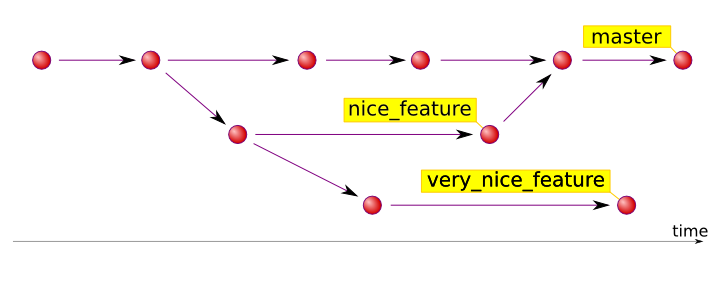
\includegraphics{git-history.png}

\begin{itemize}
\item
  Take some time to identify the commits, branching events, and merging
  events on the graph.
\item
  Note that branch names actually are names for the most recent commit
  on that branch, known as the \textbf{head} of the branch.
\end{itemize}

\begin{center}\rule{0.5\linewidth}{\linethickness}\end{center}

\begin{center}\rule{0.5\linewidth}{\linethickness}\end{center}

\subsubsection{An elementary task: cloning a remote
repository}\label{an-elementary-task-cloning-a-remote-repository}

\begin{itemize}
\tightlist
\item
  In a suitable directory, type
\end{itemize}

\begin{verbatim}
git clone git@github.com:ionides/531w18
\end{verbatim}

\begin{itemize}
\tightlist
\item
  You now have a local copy of the Stats 531 class materials. Depending
  on your setup, it may work better to use a different approach:
\end{itemize}

\begin{verbatim}
git clone https://github.com/ionides/531w18
\end{verbatim}

\begin{itemize}
\item
  The local repository remembers the address of the remote repository it
  was cloned from.
\item
  You can pull any changes from the remote repository to your local
  repository using \textbf{git pull}.
\end{itemize}

\begin{verbatim}
$ git pull
Already up-to-date.
\end{verbatim}

\begin{center}\rule{0.5\linewidth}{\linethickness}\end{center}

\begin{center}\rule{0.5\linewidth}{\linethickness}\end{center}

\subsubsection{A workflow to contribute to the 531w18 github repository:
Forking a project and making a pull
request}\label{a-workflow-to-contribute-to-the-531w18-github-repository-forking-a-project-and-making-a-pull-request}

\begin{itemize}
\item
  We will follow a standard workflow for proposing a change to someone
  else's github repository.
\item
  \textbf{Forking} is making your own github copy of a repository.
\item
  A \textbf{pull request} is a way to ask the owner of the repository to
  pull your changes back into their version.
\end{itemize}

The following steps guide you through a test example.

\begin{enumerate}
\def\labelenumi{\arabic{enumi}.}
\item
  Go to \url{http://github.com/ionides/531w18}
\item
  Click \texttt{fork} at the top right-hand corner, and follow
  instructions to add a forked copy to your own github account. It
  should now show up in your account as \texttt{my\_username/531w18}.
\item
  Clone a local copy of the forked repository to your machine, e.g.,
\end{enumerate}

\begin{verbatim}
git clone git@github.com:my_username/531w18
\end{verbatim}

Aternatively, you can type

\begin{verbatim}
git clone https://github.com/my_username/531w18
\end{verbatim}

\begin{enumerate}
\def\labelenumi{\arabic{enumi}.}
\setcounter{enumi}{3}
\item
  Move to the \texttt{531w18} directory and edit the file
  \texttt{hw0\_signup.html} to add your own name. You should use an
  ascii text editor, such as Emacs. Do not use Microsoft Word or any
  other word processing editor.
\item
  It can be helpful to type
\end{enumerate}

\begin{verbatim}
git status
\end{verbatim}

regularly to check on the current state of the repository.

\begin{enumerate}
\def\labelenumi{\arabic{enumi}.}
\setcounter{enumi}{4}
\tightlist
\item
  Commit this change to your local version of the forked
  \texttt{531w18},
\end{enumerate}

\begin{verbatim}
git add hw0_signup.html
git commit -m "sign up for my_name"
\end{verbatim}

and see how the \texttt{git\ status} has changed. Another useful command
for checking on the recent action in the repository is

\begin{verbatim}
git log
\end{verbatim}

Type \texttt{q} to exit the listing of the log.

\begin{enumerate}
\def\labelenumi{\arabic{enumi}.}
\setcounter{enumi}{5}
\tightlist
\item
  Push this change to the forked \texttt{531w18} on github:
\end{enumerate}

\begin{verbatim}
git push
\end{verbatim}

\begin{enumerate}
\def\labelenumi{\arabic{enumi}.}
\setcounter{enumi}{6}
\tightlist
\item
  On the github web site for the \texttt{my\_username/531w18} fork,
  click \texttt{New\ pull\ request} and follow instructions. When you
  have successfully placed your pull request, the owner of the forked
  repository (in this case,
  \href{mailto:ionides@umich.edu}{\nolinkurl{ionides@umich.edu}}) will
  be notified. I will then pull the modifications from your fork into
  \texttt{ionides/531w18}.
\end{enumerate}

\begin{center}\rule{0.5\linewidth}{\linethickness}\end{center}

\begin{center}\rule{0.5\linewidth}{\linethickness}\end{center}

\paragraph{Optional: upstream}\label{optional-upstream}

If you have forked and cloned the repository and would like to keep your
forked repository up to date, here is a common way of doing so:

\begin{itemize}
\item
  Go to your local repository via the terminal.
\item
  Type
  \texttt{git\ remote\ add\ upstream\ https://github.com/ionides/531w18}

  \begin{itemize}
  \tightlist
  \item
    This allows you to have 2 remote branches, `origin' which points to
    the forked repository that you have, and `upstream' which is the
    original repository. Recall that remote branches are references
    (pointers) to the state of branches in remote repositories. Thus,
    you can pull via `upstream' to update the local repository on your
    machine, then push from your updated local repository to the one on
    github.
  \end{itemize}
\item
  Type \texttt{git\ pull\ upstream\ master}. This pulls the changes in
  the upstream repository (the original repository) into the master
  branch on your local computer

  \begin{itemize}
  \tightlist
  \item
    If you have already made changes to your local repository, there
    \emph{might} be conflicts when you pull because the upsteam
    repository doesn't have those changes. You'll have to manage these
    manually if this occurs.
  \end{itemize}
\item
  Type \texttt{git\ push\ origin\ master}. This, as mentioned above,
  pushes changes from your local repository, which now contains updates
  from the original repository, to your repository on github. Now, both
  your local repository and your github repository should be updated.
\end{itemize}

\begin{center}\rule{0.5\linewidth}{\linethickness}\end{center}

\begin{center}\rule{0.5\linewidth}{\linethickness}\end{center}

\subsection*{References}\label{references}
\addcontentsline{toc}{subsection}{References}

\hypertarget{refs}{}
\hypertarget{ref-breto14}{}
Bretó, C. 2014. On idiosyncratic stochasticity of financial leverage
effects. Statistics \& Probability Letters 91:20--26.

\hypertarget{ref-ionides15}{}
Ionides, E. L., D. Nguyen, Y. Atchadé, S. Stoev, and A. A. King. 2015.
Inference for dynamic and latent variable models via iterated, perturbed
Bayes maps. Proceedings of the National Academy of Sciences of the
U.S.A. 112:719--724.


\end{document}
